\documentclass{article}
\usepackage[utf8]{inputenc}

\title{Leveraging the Criticality of Outbreaks to Eradicate Ebola}
\author{}
\date{February 9th, 2015}

\usepackage{graphicx}
\parindent 0pt
\parskip=12pt
\usepackage{float}

\usepackage[
backend=biber,
style=numeric,
sorting=none
]{biblatex}
\addbibresource{ref2.bib}
\pagenumbering{arabic}

\renewcommand{\thefootnote}{\fnsymbol{footnote}}

\usepackage{fancyhdr}
\pagestyle{fancy}
\fancyhf{}
\fancyhead[L]{Team 41825}
\fancyhead[R]{\thepage}


\usepackage[toc,page]{appendix}

\begin{document}
\maketitle

\begin{abstract}


Ebola is an extremely deadly disease that spreads rapidly through contact with infected persons. Recently, a vaccine has been developed to cure Ebola. In this paper, we discuss an optimal vaccine delivery strategy to prevent Ebola outbreaks. We consider two models for disease outbreak that have spatial dependence. Both are percolation models - models where the virus travels from the infected to the susceptible through nearest-neighbors. We examine (1) percolation on a two-dimensional lattice and (2) percolation on a small-world network, a two-dimensional lattice with random shortcuts between sites. 
In both models, we find that outbreaks exhibit critical behavior characterized by a critical vaccination density, above which outbreaks are quickly contained within an effective radius determined by this density. We also explore the effect of varying connectivity on critical density, and conclude that higher connectivity leads to a higher required critical vaccination density. In the small-world network, we compare two vaccination strategies and find that vaccination of highly connected sites does not yield a significant improvement over random vaccination. We conclude that in highly connected networks, random vaccination above a critical density, localized in a radius around the source of the Ebola outbreak is the best containment strategy, and outline a procedure that can be used to calculate this density and the resulting radius.

\end{abstract}
\clearpage

\tableofcontents
\clearpage

\section{The Terror of Ebola}
In the fall of 2014, an outbreak of Ebola spread rapidly throughout western Africa. In particular, the nations of Guinea, Liberia, and Sierra Leone found their health systems overwhelmed by the scale of the epidemic. Even with the help of international organizations such as the World Health Organization (WHO) and Doctors Without Borders (MSF), news reports of hospitals overflowing with patients continued. To give a sense of the drastic lack of resources in these countries, according to a recent report in The Economist, there are 10 doctors for every 100,000 people in Guinea \cite{Economist}. In Sierra Leone and Liberia, this number is even smaller.

This stresses the importance of economical solutions for containing an Ebola outbreak. Thus, when answering the question:``what is an optimal strategy for eradicating Ebola?" we have a few main strategic goals:
\begin{itemize}
\item Minimize the amount of vaccine that needs to be administered (and thus the number of doctors administering it).
\item Determine the most effective geographic sites for vaccine deployment to minimize transport of the vaccine.
\item Maximize the survival rate in the affected region. i.e. minimize the number of infected individuals.
\end{itemize}

\section{Searching for an Optimal Model}

Our main goal in developing a model for disease spread is to analyze vaccine-deployment strategies for containing an Ebola outbreak and preventing future outbreaks. In the following section, we examine a basic model for its deficiencies, which motivate the improved models that we develop in later sections.

\subsection{The Kermack-McKendrick Model - Blind to Connectivity}

Epidemiological modeling begins with the basic model developed by Kermack and McKendrick \cite{math_epid}. In it, a system of two differential equations describes the development of an epidemic: 
\begin{center}
$S'(t) = -\beta SI$
\\
$I'(t) = \beta SI - \alpha I$
\end{center}
Where $S(t)$ is the size of the susceptible population (i.e. those that can be infected), $I(t)$ is the size of the infected population, $\beta$ is the contact-rate, and $\alpha$ is the rate of removal (i.e. recovery rate $+$ mortality rate). 

With the contact rate $\beta$, the Kermack-McKendrick model assumes homogeneous mixing of the population; that is, each member is equally likely to come into contact (sufficient to transmit the disease) with each other member of the population. In reality, an infected individual only comes into contact with a small fraction of the population. There have been some attempts to remedy this using more complicated contact-rates \cite{math_epid}, but these models do not address the heterogeneity of human contact networks. Human networks, for example, may exhibit subgroups of highly connected individuals, and relatively sparse connections between these subgroups. We believe that including spatial heterogeneity in our model is essential to understanding and controlling a disease outbreak.
 
\subsection{Goals of the Model}
Thus we have the following goals in developing a model:
\begin{itemize}
\item Account for the heterogeneity of contact networks in disease spread.
\item Be able to compare spatially dependent vaccine-deployment strategies.
\end{itemize}

\subsection{Additional Model Assumptions}
We further simplified the problem to assume the following:
\begin{itemize}
\item The epidemiological time scale of the outbreak is small in comparison to the demographic timescale. Under this assumption, the effects of birth and natural death rates, as well as immigration/emigration, are not included. We justify this by the extreme infective nature of Ebola.
\item Outbreaks begin in highly localized regions.
\item Disease spreads along lines of human contact, i.e. not by homogeneous mixing.
\item Our vaccine is perfect: those who are vaccinated cannot be infected.
\end{itemize}

In the sections that follow, we outline two models for outbreak response to vaccination:
\begin{itemize}
\item The Site Percolation Model, where we model a human contact network as a two-dimensional lattice. 
\item The Small-world Percolation Model, where we model the human network as a partially-randomized graph.
\end{itemize}

In each, we examine the effects of vaccination outbreak containment.

\section{The Site Percolation Model}

\subsection{Simple Virus Percolation on a Lattice}
In order to get a rough picture of how a spatially distributed vaccination strategy might hinder the spread of Ebola, we employ a simple site percolation model. We model our sample population as a 2-dimensional cubic lattice, with side length $L$. Each lattice site, which could represent a single person or small, highly-connected community such as a family or neighborhood, may be initialized in one of two states, susceptible (S) or vaccinated (V). In this simplest model, the vaccine is administered randomly throughout the population, so each site is independently vaccinated with probability $\rho$, and is susceptible otherwise. Hence, on average, the density of vaccinated sites is $\rho$ while the density of susceptible sites is $1 - \rho$. 

At $t=0$, a randomly chosen susceptible site is infected, and at every subsequent time step, a susceptible site becomes infected if it has an infected nearest-neighbor. Thus, the infection percolates across the lattice, and the size of the outbreak is exactly the size of the largest connected cluster of susceptible sites, known as the ``giant component". Percolation is a quintessential critical phenomenon, and accordingly the outbreak dynamics exhibit a phase transition \cite{Sole2011}. In particular, there exists a critical vaccination density, $\rho_{c}$, where for $\rho <  \rho_{c}$, the virus percolates across the entire lattice, i.e. the outbreak becomes an epidemic, and for $\rho >  \rho_{c}$, the outbreak is contained. The critical value $\rho_{c}\approx0.4073$ \footnote{Note that in the literature, the density of interest is that of the percolating sites, rather than the sites obstructing the percolation. Hence, our $\rho$ is the complement of that seen in the literature, i.e. $\rho=1-\rho_{literature}$.} for a 2-d cubic lattice is well-known in the literature \cite{Christensen2005}, see Fig. \ref{fig:percolation}. 

\begin{figure}[H]
\centering
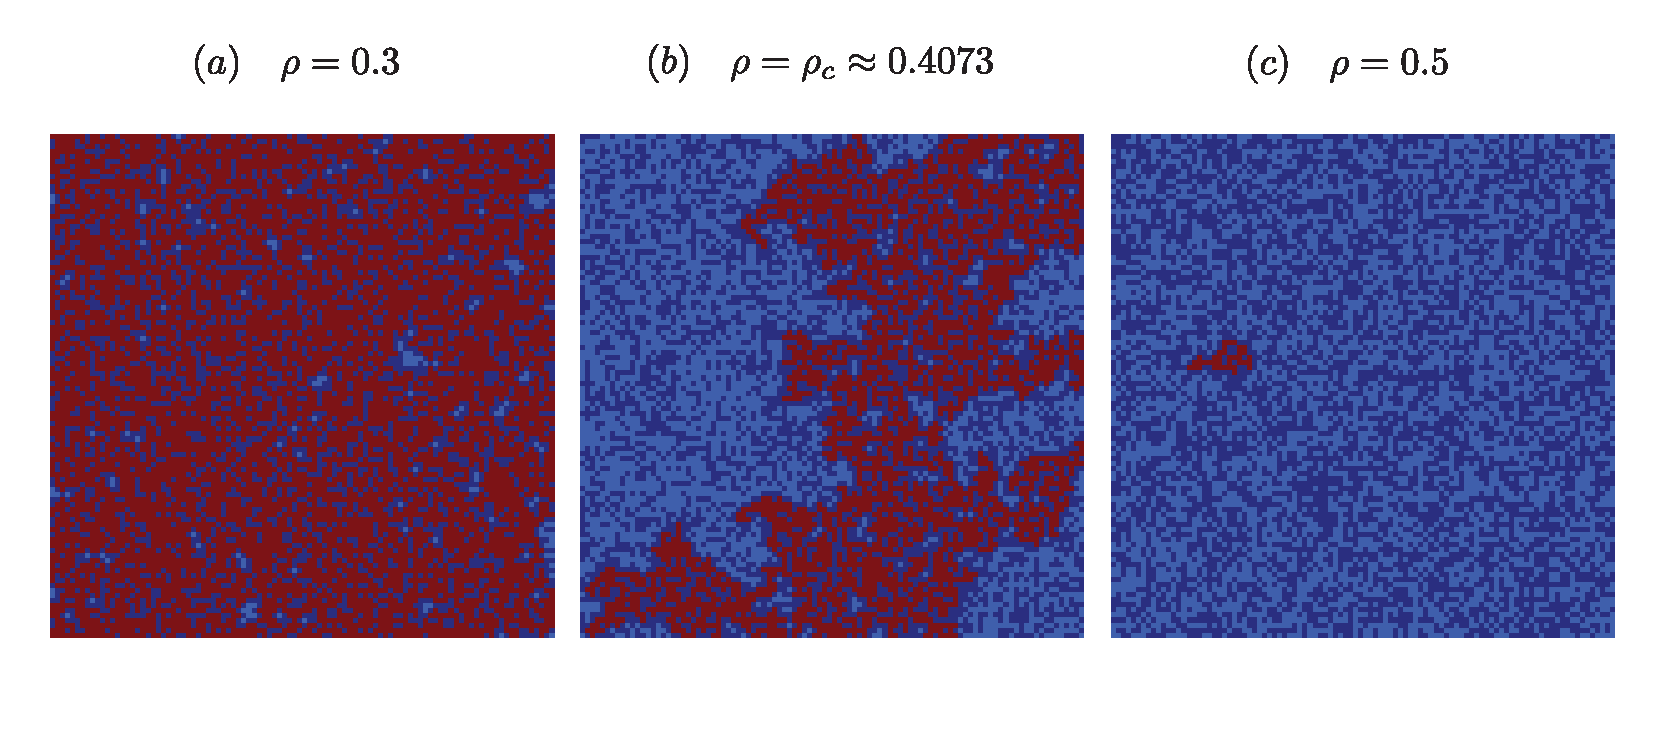
\includegraphics[scale=0.4]{figs/perc.eps}
\caption{Site percolation simulations for $L=100$. Light blue, dark blue, and red coloring indicate susceptible, vaccinated, and infected, respectively. In (a), (b), and (c) the virus dynamics are subcritical (epidemic), critical, and supercritical (contained).}
\label{fig:percolation}
\end{figure}

We take as a measure of the size of the outbreak the fraction $r$ of initially susceptible sites that become infected,
i.e. the bare infection rate. As shown in Fig. 2, this order parameter $r$ undergoes a drastic change as the critical vaccination density is crossed, characterizing the transition between the epidemic and contained phases. Moreover, the transition between these two phases becomes sharper as the lattice size increases, indicative of the approach to a thermodynamic limit, or rather an analogue thereof \cite{Goldenfeld}. 

In the subcritical phase, nearly all susceptible sites become infected, while in the supercritical phase, almost none are infected. Most importantly, within each phase, there is essentially no $\rho$ dependence on the bare infection rate $r$. This observation is the salient feature of the site percolation model; the base amount of connectivity of the 2-d lattice allows the virus to spread unimpeded in the subcritical phase, however, once the critical threshold is crossed, clusters of vaccinated sites wall in the infection, preventing any outbreak. Naively, this means the particular amount of vaccine administered in the overall population is not important provided it is above the critical amount, in this case $\rho_{c}L^{2}$.

\begin{figure}[H]
\centering
\includegraphics[scale=0.4]{figs/thermo_lim.eps}
\caption{The bare infection rate $r$ as a function of vaccination density $\rho$, simulated with 3 different lattice sizes. Each point is the average over 100 simulations. The sharpening of the phase transition is reminiscent of the approach to the thermodynamic limit, where the lattice size is infinite.}
\label{fig:Thermodynamic Limit}
\end{figure}

\subsection{A First Approach to Enhancing Connectivity}

In a real human population, individuals are not fixed in place, and in a given day tend to come into contact with other individuals from potentially distant locations. As a result, the human network becomes more connected than a simple lattice with near-neighbor interactions. The theory of so-called ``small-world" networks, pioneered by Watts and Strogatz \cite{WattsStrogatz}, aims to incorporate this enhanced connectivity, and will be applied to the site percolation model in later sections. Here, we instead model enhanced connectivity by simply extending the length of the nearest-neighbor interactions. We let $k$ be the number of steps between a site and what we consider a neighbor, computed using the usual $L_{1}$ norm, see Fig. \ref{fig:L1 norm}.

\begin{figure}[H]
\centering
\includegraphics[scale=0.4]{figs/L1norm.eps}
\caption{The location of neighbors for given $k$ values. Tagged site in black, neighbors in grey. }
\label{fig:L1 norm}
\end{figure}

Employing this enhanced nearest-neighbor interaction, we find that the virus percolation exhibits the same critical behavior with respect to the vaccination density $\rho$, but with the critical density $\rho_{c}$, as an increasing function of $k$. Fig. \ref{fig:Critical Point Shifting} shows the bare infection rate $r$ as a function of vaccination density for various $k$ values, demonstrating the shift in the epidemic-containment phase transition.  

\begin{figure}[H]
\centering
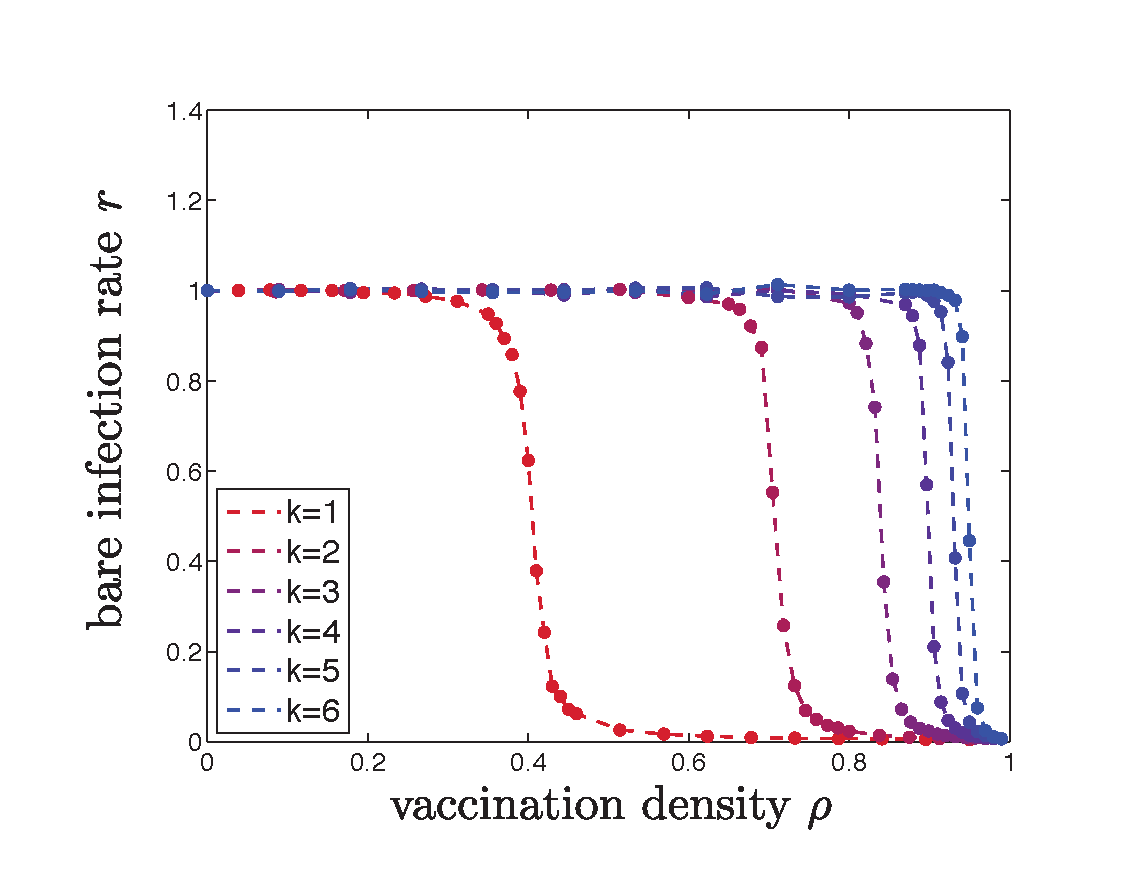
\includegraphics[scale=0.4]{figs/critical_shift.eps}
\caption{The order parameter $r$ (bare infection rate) as a function of vaccination density $\rho$, for various interaction length $k$ values. Numerical simulations were run on a lattice with $L=200$, averaged over 20 realiztions. As $k$ increases, the behavior is still critical, but with a larger critical vaccination density.}
\label{fig:Critical Point Shifting}
\end{figure}

\subsection{Outbreak Size Dynamics}

The timescale of an outbreak is also critically dependent on the vaccination density $\rho$. For example, in the simple lattice $k=1$ site percolation model, the time it takes the infection to either spread over the entire lattice or be contained is sharply peaked at the critical vaccination density, and in fact diverges in the infinite lattice limit \cite{Sole2011}. 

To investigate the more practical ramifications of this notion, we implement a modification to our lattice site percolation model where, once infected, a site remains so for a definite number of time steps, $T$, and then is removed, simulating either recovery to an immunized state, or death. As we are only concerned with the spread of outbreaks and their containment, the final fate of an infected site is not important for our analysis.\footnote{We may denote by $s$ the probability that after the illness duration $T$, the site recovers to an immune state. By varying this probability, we may lessen or increase the death toll of a given outbreak, however, this will not modulate the spatial size of the outbreak as it happens} In Fig. \ref{fig:I(t)}, we simulate the density of infected individuals $I(t)$ as a function of the time step, effectively tracking the size of the outbreak as is progresses. 

\begin{figure}[H]
\centering
\includegraphics[scale=0.4]{figs/Inf_dynamics.eps}
\caption{Density of infected individuals $I(t)$ as a function of time step during an outbreak for various values of the vaccination density $\rho$. The vaccination density increases from 0 to 1 from top to bottom, or red to blue. Each curve is the average over 100 trails for a lattice with $L=150$, and $T=3$ (see section 4.1 for a justification of this value). Note that as the critical vaccination density $\rho_{c}$ is passed the outbreak becomes supercritical, and shows exponential relaxation, similar to the phenomenological Kermack-McKendrick model.}
\label{fig:I(t)}
\end{figure}

In the subcritical phase, the dynamics of $I(t)$ show a fast increase to roughly half the lattice population, and then a decay as the infected sites either move to recovered or deceased states. Note that the integral under the curve for $\rho=0$ is not unity (it is necessarily larger), as the illness duration $T$ is larger than 1 time step. As the critical vaccination density is approached, the peak of the curve moves to larger $t$ values, and very near the critical point (purple curve), $I(t)$ is nearly flat, indicating that the outbreak duration begins to diverge, while the number of new infections equilibrates with the rate of sites recovering or perishing. Finally, in the supercritical phase, $I(t)$ shows nearly exponential decaying dynamics.\footnote{As each simulation is initialized with a single infected site, there will necessarily be an initial rapid increase in $I(t)$ as the outbreak grows into a small contained cluster} This behavior is reminiscent of the Kermack-McKendrick differential equations, which assume that the population is homogeneously mixed, i.e. all sites are neighbors.

\subsection{Average Outbreak Size}

An additional critically varying quantity in the lattice-site percolation models is the average outbreak size $\chi(\rho)$ (in our case, the number of people infected) given by the expression:

$$\chi(\rho) \propto |\rho - \rho_c|^{-\gamma}$$ 

where $\gamma$ is the so-called ``critical exponent." In the infinite lattice size limit, it can be analytically shown $\gamma = \frac{43}{18}$ \cite{Christensen2005}. Neglecting finite size effects, near $\rho_c$, the average outbreak size diverges. 

To give a sense of the improvements that can be gained near the critical point, we calculate $\eta(\alpha)$, the effectiveness of scaling the vaccination rate $\rho$ by $\alpha$ near the critical point. We write $\rho$ in terms of $\rho_c$, $\rho = \beta \rho_c$.

Assuming we are above the critical point ($\beta > 1$, and that we are increasing the vaccination rate ($\alpha > 1$), we see that:

$$
\eta(\alpha, \beta) = \frac{\chi(\rho)}{\chi(\alpha \rho)}
= \frac{|\rho - \rho_c|^{-\gamma}}{|\alpha\rho - \rho_c|^{-\gamma}}
= 
\left(\frac{|\beta\rho_c - \rho_c|}{|\alpha\beta\rho_c - \rho_c|}\right)^{-\gamma}
$$
Since $\rho_c \in [0,1]$,
$$
=
\left(\frac{|\beta - 1|}{|\alpha\beta - 1|}\right)^{-\gamma}
$$

As $\rho \rightarrow \rho_c$, $\beta \rightarrow 1$ we see that $\eta \rightarrow 0$, which we expect from the divergent size of the average outbreak at the critical point.

Assuming we are 10\% above the critical point ($\beta = 1.1$), a 10\% increase in $\rho$ yields $\eta(1.1, 1.1) = \left(\frac{0.1}{0.21}\right)^{-\gamma}$. Which, for the theoretical $\gamma = \frac{43}{18}$, yields an improvement $\eta(1.1, 1.1) \approx 5.9$. This means that a 1.1 times increase in the vaccination rate yields a \textit{6 times lower infection rate}, a huge improvement.

\subsection{Localizing Vaccine Deployment in an Effective Radius}

This characteristic outbreak size can be leveraged for strategic advantage when deploying vaccination. The size of an outbreak is the number of infected sites - on our lattice, the \textit{area} of an outbreak. On average, outbreaks are circular (i.e. don't favor any particular direction), so we can calculate an \textit{effective radius}, $R_{eff}(\rho)$ of an outbreak, relative to the size of our lattice.

$$
\chi(\rho) = \pi R_{eff}^2
$$

Which tells us that $R_{eff}$ scales with $\sqrt{\chi}$.

Strategically, this means that, if the source of an outbreak is found quickly, efforts to vaccinate the surrounding region above the critical density $\rho_c$ should be focused within a distance $\sqrt{R_{eff}}$ of the outbreak. As the density of vaccination increases above $\rho_c$, these efforts can be further localized as $R_{eff}$ decreases.


\section{Small-world Networks}
The lattice-site model suffers from one major drawback: it does not emulate the connectedness of real human networks. To address this issue, we turn to epidemic modeling on small-world networks - randomly generated graphs which emulate the random-connectedness of human contact networks \cite{Newman_Watts}.

Models of epidemics on small-world networks have been done before, and it has been shown that, on a small-world network derived from a 1-d lattice with periodic boundary conditions, focusing on vaccinating highly connected sites significantly reduces $\rho_c$ \cite{Zanette}.

In this section, we attempt to extend the results of the 1-d small-world network to a 2-d small-world network. We find that this result does not hold, and that, in fact, random vaccination performs just as well as prioritized vaccination.

\subsection{Site Percolation on a Small-world Network}

To generate the small-world network, a 2-d lattice is generated as before, but the connectivity of the lattice is then altered according to the following scheme: each edge is with probability $p$ rewired to a randomly selected site, creating a ``shortcut" through the lattice. Thus $p$ is a measure of the ``randomness" of the network, see Fig \ref{fig:p_connect}, reducing the distance between otherwise distant sites. Duplicate edges between sites are not allowed. In addition, when generating networks, disconnected graphs are not allowed.

\begin{figure}[h!]
\centering
\includegraphics[scale=0.5]{figs/increasing_p.png}
\caption{The effects of increasing $p$ on graph site connectivity on a L=20 lattice. The color of each position represents the number of connections it has. (Top left: $p$ = 0.1, Top right: $p$ = 0.21, Bottom left: $p$ = 0.46, Bottom right: $p$ = 1). Note that the per-site connectivity is still 4 on average, since no edges are lost in the randomization.}
\label{fig:p_connect}
\end{figure}

Before seeding an infection, the sites in the network are vaccinated according to one of two schemes:
\begin{itemize}
\item $\rho L^2$ sites are selected at random to be vaccinated (\textit{randomized vaccination})
\item the most connected $\rho L^2$ sites are vaccinated (\textit{prioritized vaccination})
\end{itemize}
The dynamics of percolation are the same as in the lattice model. The infection is seeded at a random site $i$. At each time step $t$, each infectious site is selected. If $T$ time has passed since the time $t_{inf}$ it was infected, i.e. $t - t_{inf} \geq T$, then the infected site is removed. In our implementation, $T = 3$, which, according to \cite{Zanette}, guarantees consistent behavior in the absence of immunization. If $t - t_{inf} < T$, the infectious site infects each of its nearest neighbors with probability $0.8$ (as opposed to 1 in the lattice model), with ``neighbor" being defined by the new connectivity of the network. If a site being infected has been previously removed, is vaccinated, or is already infected, its state does not change. The simulation proceeds until there are no more infectious sites, i.e. $I=0$. This is an absorbing state which is guaranteed, as we have a finite lattice and $I = 0$ is the only absorbing state.

The effects of increasing $p$ on the critical vaccination density can be readily seen in Fig. \ref{fig:p_rho}. Consistent with our lattice-model results, increasing connectivity - in this case, by increasing $p$ and thus decreasing the average distance between sites - results in larger values for $\rho_c$.

\begin{figure}[h!]
\centering
\includegraphics[scale=0.5]{figs/rand_immune.png}
\caption{The effects of increasing $p$ on the critical density $\rho_c$. $p$ = 0.1 (green), $p$ = 1 (red). There is a clear shift to the right of $\rho_c$ for the higher $p$ graph. Both exhibit higher critical densities than the lattice model in the previous section. Each point is the average of 50 simulations on an L=50 lattice.}
\label{fig:p_rho}
\end{figure}

\subsection{Evaluating Prioritized Vaccination on a Small-world Network}

In correspondence with the results of Zanette in \cite{Zanette}, we expected a significant improvement in $\rho_c$ for prioritized vaccination. We simulated a L=50 lattice for a wide range of parameters of $p$ and $\rho$ to examine its behavior in response to differing vaccination strategies. However, even in the most randomized networks ($p=1$), where high priority sites are much more connected than low priority sites, there was no change in $\rho_c$ for differing vaccination strategies, see Fig. \ref{fig:rand_v_prior}.

\begin{figure}[h!]
\centering
\includegraphics[scale=0.5]{figs/prior_vs_rand_p=1.eps}
\caption{The effects of vaccination strategy on the critical vaccination density $\rho_c$ for $p$ = 1. In blue, the random vaccination strategy is shown. In red, the prioritized vaccination strategy is shown. There is no significant difference in $\rho_c$. Each point is an average of 50 simulations for an L=50 lattice.} 
\label{fig:rand_v_prior}
\end{figure}

Even with the small-world randomness introduced into the lattice, the outbreaks still exhibit critical behavior (albeit with increased $\rho_c$). This implies that outbreaks on small-world networks also have a characteristic outbreak size $\chi(\rho)$, and thus, the same strategy of localized vaccine deployment (i.e. within a characteristic radius) should apply.

\section{Strengths and Weaknesses}
\paragraph{Strengths}
\begin{itemize}
\item Our models consider the spatial distribution of connections in a human network, an improvement to the homogeneous mixing of basic models.
\item Our models examine critical behavior as a function of the connectivity of the network.
\item Our models allow us to calculate an effective radius to localize vaccine deployment. This suggests a realizable strategy for vaccine deployment, discussed in the conclusion.
\end{itemize}

\paragraph{Weaknesses}
\begin{itemize}
\item Our models' main weakness is that it does not examine truly dynamic vaccine deployment. Certainly, a vaccine that can cure currently infected patients could be leveraged to achieve greater effectiveness during an outbreak.
\item Our models also do not account for diagnosis accuracy - any realistic vaccine strategy would need to account for undiagnosed cases, as well as the resource strain of false positives.
\item Our models do not take into account immigration/emigration, and therefore do not include the possibility of mass emigration due to hysteria or immigration of nearby infected people. Thus our models become less appropriate if the outbreak persists for timescales where these effects are significant.
\end{itemize}

\section{Conclusion}

In conclusion, our models found that there is a \textit{critical vaccination density}, $\rho_c$, above which an outbreak is contained. This means that an effective vaccination strategy should focus on getting above this critical density - even a small increase in vaccination density near $\rho_c$ can have huge effects on the containment of an outbreak. Conversely, a small decrease in vaccination density near $\rho_c$ can have drastic consequences for containment of an outbreak.

Furthermore, we have seen that there is a characteristic size of outbreaks. This implies that, if an outbreak is quickly diagnosed, then vaccination efforts can be localized to an \textit{effective radius} around the outbreak source.

In addition, we found that the connectivity of human networks makes an outbreak harder to contain. Realistically, if our network represents a geographic region, our finding implies that understanding its connectedness will allow us to find more realistic critical vaccination densities for effective outbreak containment.

\clearpage

\printbibliography

\clearpage

\begin{appendices}
\section{For Release by the World Medical Assocation}

The eradication of Ebola is of paramount importance to the World Medical Association.

According to our mathematical models, in order to prevent any future outbreaks, a critical proportion of the population must be vaccinated. Above this proportion, any future outbreaks will be contained within a small region. Below this proportion, an Ebola outbreak can become a raging epidemic.

Therefore, in order to prevent any future outbreaks, it is crucial that we achieve this vaccination proportion among the current population, especially in regions most at risk for an outbreak. 

However, given the limited international support for international health initiatives, our strategy is limited in vaccine production and delivery. To feasibly eradicate the current strain of Ebola, we must acknowledge the limited supply of the vaccine, as well as limited distribution. We therefore focus our efforts on priority regions - regions where recent infection has been observed. The sooner these regions are vaccinated above the critical vaccination proportional, the better chance we have of containing an outbreak.

To achieve this, we must be able to vaccinate well above the critical proportion of the region's population. For this we call on the global community to provide support in the form of financial aid and manpower, and to recognize the huge impact that a small amount of aid can have on a region whose proportion of vaccinated individuals is near this critical proportion. 

To the world community: if you witness a person showing symptoms of Ebola, report it immediately. Quickly localizing the source of an outbreak and vaccinating individuals is the most effective way to minimize its impact.

Wishing you a healthy holiday season,
\\
- The World Medical Association

\end{appendices}

\end{document}
